\section{Measurement details}
\label{app:measure}

\subsection{Protocol}
\label{sec:protocol}

We time the communication path with the training loop removed. Timing uses
on-device CUDA events with an explicit synchronisation on the pinned device, and
any diagnostic that transfers a scalar to the host is disabled, because such a
transfer synchronises the device inside the timed region. Implementations are
timed interleaved repetition by repetition rather than in
sequential blocks, so that interference from other tenants lands on all of
them at once and their ratios stay paired; the sequential design produced
swings above $100\%$ between identical configurations on this shared host. One
interleaved group holds every implementation at one agent count, including
every retained-peer count of every sparse implementation and the dense
implementations they are divided by, so a ratio never spans two groups. The
released artifacts record the dense rows with $k = N-1$, which is a label and
not a separate measurement. The primary statistic is the
minimum over samples, on the modelling assumption that contention adds time
rather than removing it, and the whole timed block is repeated so that the
spread of per-run medians is reported and not hidden
(Appendix~\ref{app:dispersion}). A minimum estimates an uncontended envelope
rather than a service time, so we checked what the choice buys: recomputing
every comparison at $192$ agents and above from the medians of the same
samples changes which implementation is faster at one of $24$ configurations,
$384$ agents with a single retained peer, where the ratio moves from $0.94$ to
$1.14$ and the group's recorded inter-run spread is $64\%$. Neither of the two
sweeps that measure the same configuration reproduces the reversal. The
pre-score path of Section~\ref{sec:prescore} is the one place where the
estimator does change a conclusion, and we report it there. GPU clocks could not be locked; the account
lacks the privilege. Operation counts are analytic, from a model that follows
the convention \texttt{torch.utils.flop\_counter} uses and that we checked
against it on the composed implementations; the hand-written kernels are outside
what that counter observes. Every count in this paper is therefore a model, and
where a count and a measurement disagree the measurement governs --- which is,
after all, the paper's subject.

Two decisions about what is compared deserve stating, because both changed our
conclusions. First, we time the attention core --- from queries, keys and values
to the message tensor --- rather than the enclosing module, since the shared
input and output projections are identical across implementations and dilute the
quantity in question. Second, the dense baseline is the better of PyTorch's
fused scaled-dot-product path and a dense attention kernel we wrote ourselves in
Triton, with the same tiling policy and in the same session as the sparse
kernels. At the head widths multi-agent communication uses, the library path is
tuned for a different regime, and comparing a hand-written sparse kernel against
it credits sparsity with the difference between two authors
(Section~\ref{sec:pitfalls}).

Every implementation is checked against the reference at every configuration
whose latency any artifact reports --- $158$ of them, $136$ with $k < N-1$ so
that selection is exercised. This is not a formality: exact top-$k$ is
discontinuous in the scores, so two implementations that accumulate the score
product in different orders can rank a near-tied pair differently and then
aggregate over different peers. All agree to \texttt{fp32} rounding except on
four query rows in $1.25$ million, where two scores tie exactly at the $k$-th
position and the threshold-selecting kernel keeps one extra peer
(Appendix~\ref{app:verification}).

Unless stated otherwise: PyTorch 2.11 with CUDA 12.8 and Triton 3.6,
\texttt{fp32}, head width $d{=}16$, batch $256$, and one NVIDIA Blackwell GPU
shared with other tenants.


\subsection{The fused crossover and three selection strategies}
\label{app:selection}

\begin{table}[t]
\centering\small
\caption{The sparsity at which the best sparse implementation stops being faster than the best dense one, and how far it is from parity at a quarter of the peers. Both ratio columns are a minimum over the composed path and the two fused kernels that rank in registers, so the widest-$k$ column is sometimes the composed path; the sorted kernel of Table~\ref{tab:selection} is faster than all three from sixteen retained peers upward and is reported there. Restricted to the agent counts at which per-kernel cost does not dominate. The replayed column is the fused kernel at one retained peer under CUDA-graph replay, pooled over three further sessions of three interleaved blocks each, as ratio of minima and ratio of medians.}
\label{tab:crossover}
\begin{tabular}{rccrrcrr}
\toprule
& \multicolumn{2}{c}{\textbf{sparsity that pays}} &
  \multicolumn{2}{c}{\textbf{best ratio}} &
  \textbf{replayed, $k{=}1$} &
  \multicolumn{2}{c}{\textbf{at the widest $k$}} \\
\cmidrule(lr){2-3}\cmidrule(lr){4-5}\cmidrule(lr){6-6}\cmidrule(lr){7-8}
$N$ & $k$ & of peers & ratio & at $k$ & min / median & ratio & at $k$ \\
\midrule
192 & $\le 1$ & 0.5\% & 0.76 & 1 & 0.76 / 0.77 & 27.9 & 128 \\
384 & $\le 1$ & 0.3\% & 0.94 & 1 & 0.92 / 0.92 & 18.8 & 128 \\
512 & $\le 1$ & 0.2\% & 0.81 & 1 & 0.77 / 0.77 & 15.4 & 128 \\
\bottomrule
\end{tabular}%

\end{table}

That statement has to be qualified in turn, and the qualification is the more
useful result. Matched authorship is a weaker condition than matched efficiency:
two kernels written by the same person in the same session can still differ by
more than the margin being measured, and only efficiency against the machine
identifies the algorithm. We therefore searched the same parameter space for
both kernels under the same admissibility filter, took the better of that search
and the vendor library as the dense baseline, and report what fraction of the
device's own matrix-multiply rate each kernel reaches beside its latency
(Table~\ref{tab:autotune}).

\begin{table}[t]
\centering\small
\caption{Both kernels searched over one parameter space --- query tile, key tile
or head chunk, warp count and pipeline depth --- under one shared-memory
admissibility filter, with the better of the search and the vendor library taken
as the dense baseline. The \emph{cfgs} columns are how many configurations each
search admitted; the sparse kernel must hold an $N$-wide score tile, so above
$192$ agents only three fit. Efficiency is executed arithmetic over elapsed time,
against the matrix-multiply rate the device attains in the same process. These
are the search session's own timings, taken configuration by configuration
rather than interleaved; the two search sessions measured peaks of $58$ and
$71$~TFLOP/s, so the efficiency columns are comparable within a row but not
across sessions. Every ratio elsewhere in the paper re-times the selected
configurations in an interleaved sweep.}
\label{tab:autotune}
\resizebox{\linewidth}{!}{\begin{tabular}{rr lrrr rrrr r c}
\toprule
& & \multicolumn{4}{c}{\textbf{best dense}} &
    \multicolumn{4}{c}{\textbf{best sparse}} & & \\
\cmidrule(lr){3-6}\cmidrule(lr){7-10}
$d$ & $N$ & from & cfgs & ms & \% peak & $k$ & cfgs & ms & \% peak & ratio
& $k$ that pays \\
\midrule
16 & 192 & triton & 106 & 0.0347 & 30 & 1 & 12 & 0.0249 & 21 & 0.72 & $\le 1$ \\
16 & 384 & triton & 106 & 0.1082 & 38 & 1 & 3 & 0.0941 & 22 & 0.87 & $\le 1$ \\
16 & 512 & triton & 106 & 0.1681 & 44 & 1 & 3 & 0.1293 & 29 & 0.77 & $\le 1$ \\
32 & 192 & triton & 94 & 0.0555 & 38 & 1 & 18 & 0.0428 & 24 & 0.77 & $\le 1$ \\
32 & 384 & triton & 94 & 0.1923 & 43 & 1 & 3 & 0.1618 & 26 & 0.84 & $\le 1$ \\
32 & 512 & triton & 94 & 0.3179 & 47 & 1 & 3 & 0.2231 & 33 & 0.70 & $\le 2$ \\
64 & 192 & sdpa & 64 & 0.0862 & 48 & 1 & 21 & 0.0962 & 22 & 1.12 & none \\
64 & 384 & sdpa & 64 & 0.2720 & 61 & 1 & 3 & 0.4321 & 19 & 1.59 & none \\
64 & 512 & sdpa & 64 & 0.4361 & 68 & 1 & 3 & 0.5634 & 26 & 1.29 & none \\
128 & 192 & sdpa & 28 & 0.1665 & 50 & 2 & 18 & 0.1724 & 24 & 1.04 & none \\
128 & 384 & sdpa & 28 & 0.4688 & 71 & 1 & 3 & 0.8582 & 19 & 1.83 & none \\
128 & 512 & sdpa & 28 & 0.7656 & 77 & 1 & 3 & 1.1784 & 25 & 1.54 & none \\
\bottomrule
\end{tabular}%
}
\end{table}

The search is not equal. All three of our sparse kernels keep the whole score
row of a query resident --- two rank it in registers and one sorts it in place
--- so their resident tile grows with the agent count, and above $192$ agents
the shared-memory filter admits only three configurations against the dense
kernel's twenty-eight to a hundred and six. That is a property of these kernels and not
of exact top-$k$: the streaming kernel of Section~\ref{sec:fused} computes all
$N$ scores without holding them and admits the dense kernel's tilings, so the
search counts here describe the resident kernels only. We
report the counts in the table rather than describing the two searches as
equivalent, and the consequence runs in two directions. The sparse kernel's
efficiency figure is a lower bound on what a sparse kernel of this shape could
reach, so the negative entries at head width $64$ and above are weakly supported
and we do not build on them. The positive entry is conservative for the same
reason: an under-searched sparse kernel that is nonetheless faster is faster.

With that said, two things follow.

The crossover survives tuning, and it is not produced by a sparse kernel that
happens to be well written. Across head widths $16$ and $32$ the sparse kernel
is the \emph{less} efficient of the two at every agent count --- $21$ to $33\%$
of the device's rate against $30$ to $47\%$ for dense --- and it is faster only
because it performs about half the arithmetic.

The crossover is an existence result inside a stated envelope, and the envelope
is narrow: one GPU architecture, \texttt{fp32}, head widths $16$ and $32$, agent
counts from $192$ upward where the sweep reproduces, a single retained peer with
one configuration at two, and a dense baseline that reaches under half of the
device's arithmetic rate at those head widths. At four retained peers the resident
kernel is already $1.3$ to $2.3$ times slower, and at a quarter of peers it is
more than an order of magnitude slower; the streaming kernel of
Section~\ref{sec:fused} moves the boundary to between two and four retained
peers. The $k{=}1$ case is also degenerate as
an attention mechanism, because a softmax over one element is identically one
and the mechanism reduces to copying the highest-scoring peer's value. What the
crossover establishes is that the penalty measured earlier is not irreducible;
it is not a recommendation to sparsify.

Why it is confined to narrow heads could not be decided from the fp32 data
alone. Dense efficiency and head width move together there --- $30\%$ at
$d{=}16$ rising to $77\%$ at $d{=}128$, as the score product becomes a
better-shaped matrix multiply --- so ``the crossover disappears once dense
attention is near the machine'' and ``the crossover disappears above $d{=}32$''
fit it equally well. The precision study of Section~\ref{sec:precision}
separates them: at a fixed head width, a dense kernel that uses the tensor cores
removes the crossover from $384$ agents upward, which supports the first
reading.

\begin{table}[t]
\centering\small
\caption{Three ways of reaching the same retained set, at the two agent counts
that carry the crossover. Repeated argmax keeps the aggregation sparse and pays
linearly in the number retained; bisecting on the score's bit pattern is flat in
it and pays the dense aggregation; sorting score--index pairs once is flat and
sparse at the same time, and is not competitive with either at the agent counts
where a sort no longer fits alongside a useful block of queries.}
\label{tab:selection}
\begin{tabular}{rr rr rr rr}
\toprule
& & \multicolumn{2}{c}{\textbf{$k$ argmax rounds}}
& \multicolumn{2}{c}{\textbf{bisection}}
& \multicolumn{2}{c}{\textbf{one sort}} \\
\cmidrule(lr){3-4}\cmidrule(lr){5-6}\cmidrule(lr){7-8}
$N$ & $k$ & ms & $\div$dense & ms & $\div$dense & ms & $\div$dense \\
\midrule
192 & 1 & 0.026 & 0.8 & 2.392 & 69.4 & 0.164 & 4.7 \\
 & 2 & 0.045 & 1.3 & 2.435 & 70.7 & 0.166 & 4.8 \\
 & 4 & 0.069 & 2.0 & 2.435 & 70.7 & 0.168 & 4.9 \\
 & 8 & 0.116 & 3.4 & 2.435 & 70.7 & 0.173 & 5.0 \\
 & 16 & 0.206 & 6.0 & 2.441 & 70.8 & 0.185 & 5.4 \\
 & 32 & 0.385 & 11.2 & 2.440 & 70.8 & 0.223 & 6.5 \\
\midrule
512 & 1 & 0.139 & 0.8 & 2.970 & 17.2 & 2.433 & 14.1 \\
 & 2 & 0.217 & 1.3 & 2.716 & 15.8 & 2.450 & 14.2 \\
 & 4 & 0.337 & 2.0 & 2.764 & 16.0 & 2.493 & 14.5 \\
 & 8 & 0.557 & 3.2 & 2.912 & 16.9 & 2.490 & 14.5 \\
 & 16 & 1.002 & 5.8 & 2.911 & 16.9 & 2.316 & 13.4 \\
 & 32 & 1.884 & 10.9 & 2.920 & 16.9 & 2.651 & 15.4 \\
\bottomrule
\end{tabular}%

\end{table}

Selection is what a successor design has to face, and we tried three ways of
doing it. Ranking $N$ candidates to keep $k$ by repeated argmax costs $k$
sequential row-wide reductions, and a reduction of that shape runs at a small
fraction of the arithmetic units' throughput because each round depends on the
one before it and the hardware has nothing to overlap it with. That is why the
argmax kernel's cost grows almost linearly in $k$ while its arithmetic barely
does. Bisecting on the score's bit pattern removes the dependence on $k$, and
the only way it can is by expressing the retained set as a zero weight instead
of by compaction --- so it performs the dense aggregation arithmetic whatever
$k$ is.

Whether both can be had at once is the obvious question, and they can
(Table~\ref{tab:selection}). Packing each score against its own peer index in
one machine word and sorting the row once yields the retained peers already
compacted: the aggregation then reads exactly $k$ value rows, while selection
costs a single bitonic sort, whose depth grows with the agent count alone and
not at all with $k$. That is visible in what the kernel costs. At $192$ agents
it runs in $0.164$\,ms at one retained peer and $0.185$\,ms at sixteen, a rise
of thirteen per cent, against an eightfold rise for the argmax kernel over the
same range; what remains of the growth is the aggregation, which is linear in
$k$ by construction, and not the selection.

It is also five times the cost of dense attention across that whole range, and
it overtakes the argmax kernel only at sixteen retained peers, where both
already cost more than five times dense. At $384$ and $512$ agents it is worse
still, thirteen to sixteen times dense at every sparsity below thirty-two
retained peers, because a row-wide sort needs the whole score row resident and
the block of queries that can share a program shrinks as the row grows. Having
both properties does not help. The sort that buys independence from $k$ costs
more than the argmax rounds it replaces throughout the range in which sparsity
would otherwise pay.

The second obstacle is one dense attention avoids and none of the resident-row
kernels does. Dense attention streams keys and values in blocks under an online softmax,
keeping a small tile resident whatever $N$ is. Each of those kernels
instead holds the $N$-wide score row --- in registers to rank it, or in place to
sort it --- so fewer queries can be in flight per streaming multiprocessor as
$N$ grows, and the tiling the search chooses for it is narrower at every size.
What is fundamental to exact score-then-select is that all $N$ scores must be
\emph{computed} before the retained set is known; that they must all be
\emph{resident} is not, and a streaming exact top-$k$ that keeps a running
candidate set relaxes it. The streaming kernel of Section~\ref{sec:fused} does
exactly that, and is faster than every resident kernel at every configuration
both cover (Table~\ref{tab:streaming}).


\subsection{The streaming kernel in reduced precision}
\label{app:streamprec}

\begin{table}[t]
\centering\small
\caption{The streaming kernel of Table~\ref{tab:streaming} in reduced
precision, searched separately in each format, against the best dense
implementation of the same format and interleaved sweep (ratios of minima under
CUDA-graph replay); the resident kernel at one retained peer is re-timed in the
same sweep. A dash marks a configuration in which TF32 rounding changed the
retained set in more than $0.1\%$ of query rows; bf16 changed none.}
\label{tab:streamprec}
\begin{tabular}{lrrcccc}
\toprule
& & & \multicolumn{3}{c}{\textbf{streaming}, $\div$ best dense} & \textbf{resident} \\
\cmidrule(lr){4-6}
format & $d$ & $N$ & $k{=}1$ & $k{=}2$ & $k{=}4$ & $k{=}1$ \\
\midrule
TF32 & 16 & 192 & 0.82 & 1.01 & --- & 0.90 \\
 & 16 & 384 & 0.78 & --- & --- & 1.08 \\
 & 16 & 512 & 0.73 & --- & --- & 1.10 \\
 & 32 & 192 & 0.70 & 0.88 & --- & 0.83 \\
 & 32 & 384 & 0.62 & 0.78 & --- & 1.32 \\
 & 32 & 512 & 0.62 & --- & --- & 1.28 \\
\midrule
bf16 & 16 & 192 & 1.06 & 1.34 & 2.09 & 1.06 \\
 & 16 & 384 & 0.99 & 1.58 & 2.61 & 1.33 \\
 & 16 & 512 & 0.96 & 1.66 & 2.71 & 1.10 \\
 & 32 & 192 & 0.96 & 1.14 & 1.76 & 0.93 \\
 & 32 & 384 & 0.92 & 1.15 & 2.02 & 1.39 \\
 & 32 & 512 & 0.85 & 1.10 & 1.92 & 1.22 \\
\bottomrule
\end{tabular}%

\end{table}

\subsection{Sensitivity to head width and batch}
\label{sec:sensitivity}


Across head widths to $512$, and at the agent counts from $192$ upward that
carry claims, the crossover exists only at the two narrowest: the best sparse
implementation is faster than the best dense one at head widths $16$ and $32$
at every agent count, and at no agent count for head width $64$ or above, where
it is $1.3$ to $2.3$ times slower (Appendix~\ref{app:grid}). The launch-bound
$96$-agent column has one exception, $0.88$ at head width $64$, which we do not
read as a result. The ratio does not fall monotonically with head
width; it reverses.

That is what the byte criterion predicts. Byte-neutrality requires
$kd \le N$, so widening the head at fixed agent count tightens the bound on the
retained set proportionally, and at head width $128$ the criterion permits only $k \le 4$ at $512$ agents (exactly $k \le 3$) --- by which point the selection cost of
Section~\ref{sec:fused} has already overtaken the saving. Widening the batch
over a
thirty-twofold range, by contrast, moves the ratio by up to a third --- from
$0.54$ to $0.72$ at $512$ agents --- and never across parity, which is the expected behaviour of a quantity that is a
ratio of per-element costs.


\subsection{Other GPU generations}
\label{app:portability}

\begin{table}[t]
\centering\small
\caption{The headline quantities on four GPUs. Each device's tilings are
searched on that device before any sweep times them, and each quantity is
computed by the function that computes it for the main text
(\texttt{scripts/summarise\_portability.py}); every entry is a ratio against the
best dense implementation of the same interleaved sweep, so a value below one
means the sparse path is faster. Streaming ranges are over $d \in \{16, 32\}$
and the agent counts of Table~\ref{tab:streaming}, under CUDA-graph replay;
the other rows are defined as in the main-text tables they summarise. The
Blackwell card was shared with other tenants; the other three were allocated
exclusively, one GPU per job, on a shared node. The A100 runs PyTorch 2.11 and
Triton 3.6 built against CUDA 12.9, the others the same versions built against
CUDA 12.8.}
\label{tab:portability}
\resizebox{\linewidth}{!}{\begin{tabular}{lcccc}
\toprule
& \shortstack{RTX PRO 6000\\(sm\_120)} & \shortstack{A100\\(sm\_80)} & \shortstack{H100 SXM\\(sm\_90)} & \shortstack{H200\\(sm\_90)} \\
\midrule
\multicolumn{5}{l}{\emph{Time $\div$ best dense, same format (lower is better)}} \\
Composed, fp32, forward, best & 9.01 & 6.57 & 6.75 & 7.65 \\
Composed, fp32, backward, best & 1.53 & 2.60 & 2.03 & 2.10 \\
Resident, fp32, $k{=}1$ & 0.67--0.91 & 0.69--0.87 & 0.69--0.89 & 0.69--0.89 \\
Streaming, fp32, $k{=}1$ & 0.46--0.63 & 0.56--0.64 & 0.56--0.68 & 0.56--0.68 \\
Streaming, fp32, $k{=}2$ & 0.56--0.84 & 0.77--0.96 & 0.76--1.13 & 0.76--1.13 \\
Streaming, fp32, $k{=}4$ & 0.78--1.15 & 1.03--1.50 & 1.05--1.45 & 1.05--1.47 \\
Streaming, fp32, $k{=}8$ & 0.92--1.76 & 1.28--2.96 & 1.25--2.04 & 1.25--2.06 \\
Streaming, TF32, $k{=}1$ & 0.62--0.82 & 0.83--1.05 & 0.83--1.03 & 0.88--1.33 \\
Streaming, bf16, $k{=}1$ & 0.85--1.06 & 1.03--1.30 & 1.10--1.32 & 1.11--1.52 \\
Z-order, fp32: attend; total & 0.09; 0.85 & 0.22; 1.22 & 0.24; 1.45 & 0.16; 1.12 \\
\midrule \multicolumn{5}{l}{\emph{Where the time goes}} \\
Resident: finding the set & 90--95\% & 91--95\% & 91--96\% & 93--97\% \\
Streaming: finding the set & 85--91\% & 88--94\% & 88--94\% & 88--95\% \\
$N{\le}96$: $\rho$ kernels; $\rho$ ops & 0.95; 0.03 & 0.91; 0.10 & 0.94; 0.02 & 0.93; 0.06 \\
\bottomrule
\end{tabular}%
}
\end{table}

\begin{table}[t]
\centering\small
\caption{The streaming kernel against the best dense implementation as the
batch varies, $d{=}16$, agent counts $192$ to $512$, both kernels searched at
every batch (ratios of minima under CUDA-graph replay). Heads are independent,
so $H$ heads over a batch $B$ are one launch over a batch $BH$: this is also the
multi-head packing sweep.}
\label{tab:portbatch}
\resizebox{\linewidth}{!}{\begin{tabular}{rccccccccc}
\toprule
& \multicolumn{3}{c}{A100 (sm\_80)} & \multicolumn{3}{c}{H100 SXM (sm\_90)} & \multicolumn{3}{c}{H200 (sm\_90)} \\
\cmidrule(lr){2-4}\cmidrule(lr){5-7}\cmidrule(lr){8-10}
$B$ & $k{=}1$ & $k{=}2$ & $k{=}4$ & $k{=}1$ & $k{=}2$ & $k{=}4$ & $k{=}1$ & $k{=}2$ & $k{=}4$ \\
\midrule
32 & 0.60--1.08 & 0.86--1.86 & 1.41--1.83 & 0.71--1.17 & 1.00--1.00 & 1.45--1.90 & 0.71--0.76 & 0.95--1.24 & 1.34--1.94 \\
256 & 0.58--0.64 & 0.87--0.96 & 1.29--1.50 & 0.61--0.65 & 0.86--0.94 & 1.35--1.45 & 0.61--0.64 & 0.85--0.94 & 1.35--1.47 \\
1024 & 0.57--0.62 & 0.87--0.91 & 1.26--1.40 & 0.60--0.64 & 0.86--0.87 & 1.36--1.40 & 0.60--0.64 & 0.86--0.87 & 1.37--1.40 \\
4096 & 0.57--0.60 & 0.83--0.88 & 1.22--1.38 & 0.59--0.62 & 0.84--0.85 & 1.32--1.39 & 0.59--0.62 & 0.84--0.85 & 1.32--1.39 \\
\bottomrule
\end{tabular}%
}
\end{table}

We repeated the measurements of Section~\ref{sec:measurement} on an A100-SXM4
(40\,GB, sm\_80), an H100 SXM (80\,GB HBM3, sm\_90) and an H200 (141\,GB HBM3e,
sm\_90), with every tiling searched again on each device
(\texttt{scripts/run\_portability\_campaign.sh}). Table~\ref{tab:portability}
collects the quantities the main text rests on. The ordering holds on all
\PortDevices{} devices: the composed path is at least \PortComposedMin{} times
slower than dense attention; from $384$ agents upward \PortFindLo{} to
\PortFindHi{}\% of the fused kernel's time is finding the set; and the streaming
kernel is faster than dense at one retained peer in fp32 (\PortStreamOneLo{} to
\PortStreamOneHi{}). Beyond that the streaming kernel's advantage shrinks. At two retained peers the
streaming kernel ranges from \PortStreamTwoLo{} to \PortStreamTwoHi{}, so it is
no longer faster at every configuration; at four it is slower everywhere
(\PortStreamFourLo{} to \PortStreamFourHi{}). At one retained peer it costs
\PortTfOneLo{} to \PortTfOneHi{} times dense in TF32 and \PortBfOneLo{} to
\PortBfOneHi{} in bf16, so in bf16 it does not break even on any of the three.
The Z-order pre-score path at $512$ agents and four retained peers is not
faster on any of them: its fused attention stage costs \PortZorderAttendLo{} to
\PortZorderAttendHi{} times dense, but with the selector the path costs
\PortZorderTotalLo{} to \PortZorderTotalHi{}. The resident kernel's one-peer ratio is
the same on all four devices; for the streaming kernel and the pre-score path
the Blackwell card is the most favourable of the four, and the crossovers the
main text reports for them are best cases.

\paragraph{Batch and heads.} Table~\ref{tab:portbatch} varies the batch from
$32$ to $4096$ on the three devices. From $256$ upward the threshold does not
move: at one retained peer the streaming kernel costs \PortBatchOneLo{} to
\PortBatchOneHi{} times dense and at two \PortBatchTwoLo{} to \PortBatchTwoHi{}.
At a batch of $32$, where a launch has only a few programs per
multiprocessor, the one-peer ratio widens to \PortBatchSmallOneLo{} to \PortBatchSmallOneHi{}. Packing more
heads into a launch therefore cannot widen the window; it can only bring a small
batch back to the large-batch ratio.

\paragraph{Hardware counters.} On the H100 and the H200 we recorded Nsight
Compute counters for every kernel each implementation launches
(\texttt{scripts/ncu\_counters.py}; the A100 nodes do not expose the profiling
counters to users). At $512$ agents and four retained peers the composed path
moves \PortNcuComposedGB{}\,GB through DRAM in \PortNcuKernels{} kernels,
against \PortNcuDenseMB{}\,MB for the tuned dense kernel; \PortNcuSelectKernels{}
of those kernels are \texttt{torch.topk}'s multi-block radix select, which makes
four passes over the score matrix and takes \PortNcuSelectShareLo{} to
\PortNcuSelectShareHi{}\% of the path's time. The composed baseline is thus
already a production radix top-$k$, and its cost is the byte criterion's:
compaction adds traffic. The fused and streaming kernels move about as many
bytes as dense attention and reach only \PortNcuFusedDramLo{} to
\PortNcuFusedDramHi{}\% of peak DRAM throughput, against \PortNcuFusedSmLo{} to
\PortNcuFusedSmHi{}\% of peak SM throughput. Selection inside a fused kernel
is bound on the multiprocessors, not by bandwidth, which is consistent with the
H200, with \PortBwRatioHTwoHundred{} times the H100's measured DRAM bandwidth, giving the same
ratios.

\subsection{Where the time goes}
\label{sec:stages}\label{app:stages}


\begin{table}[t]
\centering\small
\caption{Per-stage accounting for both paths at $N{=}\StagesN$. The
last column is the fraction of whichever machine limit binds the stage, and it
separates a stage that is badly implemented from one doing the only thing its
access pattern permits. The byte counts are analytic and count each tensor
once, so a figure above $100\%$ marks a stage whose working set is partly
served from cache. That happens for the softmax stages here and, at smaller
agent counts, for the gather; it bounds the model's error at around $+50$
percentage points, which is larger than several of the gaps in the column and
is why we do not read small differences off it.
\StagesCaption}
\label{tab:stages}
\begin{tabular}{lrrrrrrr}
\toprule
\textbf{stage} & GFLOP & GB & FLOP/byte & ms & TFLOP/s & GB/s & \% of limit \\
\midrule
score product & 2.15 & 0.29 & 7.53 & 0.549 & 3.91 & 520 & 35 \\
softmax over $N$ & 0.34 & 0.54 & 0.62 & 0.336 & 1.00 & 1598 & 107 \\
dense aggregation & 2.15 & 0.29 & 7.53 & 0.235 & 9.13 & 1213 & 81 \\
top-$k$ selection & 0.00 & 0.47 & --- & 3.271 & --- & 143 & 10 \\
softmax over $k$ & 0.08 & 0.13 & 0.62 & 0.059 & 1.42 & 2268 & 151 \\
gather of $V$ & 0.00 & 1.21 & --- & 0.954 & --- & 1265 & 84 \\
sparse aggregation & 0.53 & 1.14 & 0.47 & 0.816 & 0.65 & 1398 & 93 \\
\bottomrule
\end{tabular}%

\end{table}

\begin{figure}[t]
\centering
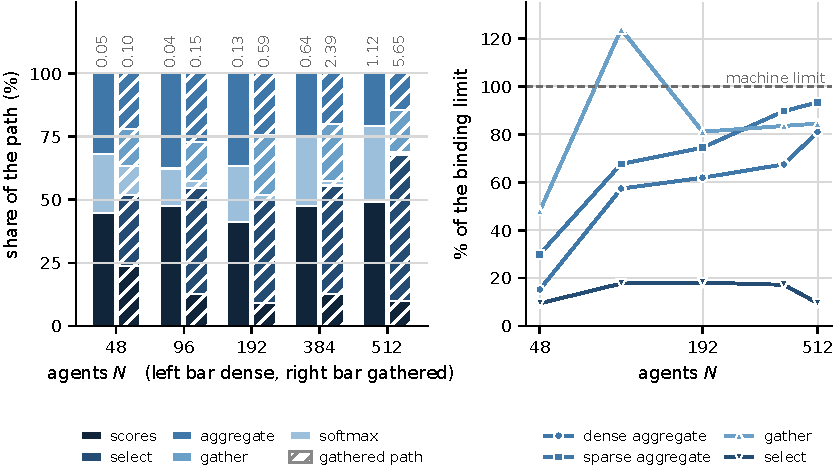
\includegraphics[width=\linewidth]{figures/fig3_stages.pdf}
\caption{\textbf{Left:} how each path divides its time. Selection grows to
dominate the gathered path as the agent count rises. \textbf{Right:} how close
each stage runs to the machine limit that binds it.}
\label{fig:stages}
\end{figure}

Low arithmetic intensity in a batched matrix--vector product is the natural
explanation for the sparse contraction's slowness, and it is not the right one.
Timed in isolation and charged with its own arithmetic and traffic, both
aggregations sit near the bandwidth the device attains on a large copy ---
$93\%$ for the sparse contraction and $81\%$ for the dense multiply it
replaces (Table~\ref{tab:stages}). The gap between them is smaller than the
byte model's own
error, so the model cannot order the two; what it does establish is that neither
sits on a worse hardware path. The sparse one is slower because it moves about
four times the bytes, since the compacted operand carries $kd$ elements per
query where the
score row carries $N$. The corrected account is simpler, checkable before the
code is written, and it is the $kd \le N$ criterion of Section~\ref{sec:roofline}.

Selection is a different case, and it is the one stage where the raw
decomposition is misleading in the opposite direction. It is the largest stage
of the composed sparse path, and it runs at under a tenth of the bandwidth the
device attains: it must read the score matrix and write values and indices, and
moving those bytes and nothing else would take a small fraction of the time it
does. That headroom is real, and the fused kernels realise part of it. What no
kernel removes is that the score matrix must be formed and ranked at all, and
the fused measurements of Section~\ref{sec:fused} show what remains once the
headroom is taken.


\subsection{Backward pass and training throughput}
\label{sec:backward}\label{app:backward}


\begin{table}[t]
\centering\small
\caption{Forward, backward and their sum, for the differentiable implementations. The
sparse path's backward is cheap relative to its forward, because selection has
almost no adjoint, so the gap against fused dense narrows without closing.
Restricted to the agent counts that reproduce: below $192$ the forward and the
forward-plus-backward passes are timed in separate interleaved blocks, and the
contention between blocks exceeds the backward's own cost, which at two
configurations produced a difference a backward pass cannot have.}
\label{tab:backward}
\resizebox{\linewidth}{!}{\begin{tabular}{rr rrr rrr rrr rrr r}
\toprule
& & \multicolumn{3}{c}{dense, unfused} & \multicolumn{3}{c}{dense, fused}
& \multicolumn{3}{c}{top-$k$ masked} & \multicolumn{3}{c}{top-$k$ gathered} & \\
\cmidrule(lr){3-5}\cmidrule(lr){6-8}\cmidrule(lr){9-11}\cmidrule(lr){12-14}
$N$ & $k$ & f & b & f+b & f & b & f+b & f & b & f+b & f & b & f+b
& \begin{tabular}[b]{@{}c@{}}gathered f+b\\$\div$ fused f+b\end{tabular} \\
\midrule
192 & 32 & 0.136 & 0.166 & 0.302 & 0.072 & 0.219 & 0.291 & 0.454 & 0.460 & 0.914 & 0.424 & 0.201 & 0.625 & 2.1 \\
384 & 64 & 1.082 & 1.604 & 2.686 & 0.220 & 0.728 & 0.948 & 3.065 & 3.365 & 6.430 & 2.405 & 1.593 & 3.998 & 4.2 \\
512 & 128 & 1.899 & 2.648 & 4.547 & 0.349 & 1.203 & 1.552 & 6.985 & 5.748 & 12.734 & 6.435 & 3.142 & 9.577 & 6.2 \\
\bottomrule
\end{tabular}%
}
\end{table}

Every latency reported so far is a forward pass, which for a training claim is
half the question. Timing forward and backward under the same protocol leaves
the ordering intact and roughly a third of the margin
(Table~\ref{tab:backward}). The gathered path's backward costs about half its
own forward, because the
expensive stage --- selection --- has almost no adjoint: the retained indices are recorded in the forward pass, and the backward is a scatter of gradients into the retained positions followed by two dense products. Dense attention's backward costs several times its forward. At
$512$ agents the gathered path is $18.4$ times the fused dense path on the
forward alone and $6.2$ times on forward and backward together, and the same
narrowing appears at every agent count in the table. The sparse path's
disadvantage in training is therefore substantially smaller than the
forward-only measurements suggest, and remains a disadvantage. The fused
kernels are excluded from this comparison: they are
hand-written forward passes, and timing one against an autograd graph would
compare two different things.

\begin{table}[t]
\centering\small
\caption{Where one MAPPO iteration spends its time. Differences between
communication implementations are at or below the iteration-to-iteration spread
in the rightmost column.}
\label{tab:trainstep}
\resizebox{\linewidth}{!}{\begin{tabular}{ll rrrrr rrr}
\toprule
& & \multicolumn{5}{c}{\textbf{share of the iteration (\%)}} & & & \\
\cmidrule(lr){3-7}
$N$ & communication & environment & acting & update fwd & update bwd & optimiser & s/iter & $\div$ fused & spread \\
\midrule
6 & none & 49 & 29 & 11 & 6 & 4 & 2.11 & 1.002 & 4.6 \\
6 & dense, unfused & 48 & 30 & 12 & 6 & 4 & 2.09 & 0.992 & 7.3 \\
6 & dense, library fused & 48 & 30 & 12 & 6 & 4 & 2.10 & 1.000 & 4.0 \\
6 & top-$k$, masked & 48 & 30 & 12 & 6 & 4 & 2.09 & 0.996 & 5.4 \\
6 & top-$k$, gathered & 49 & 29 & 12 & 6 & 4 & 2.13 & 1.011 & 5.3 \\
12 & none & 76 & 14 & 5 & 2 & 2 & 4.35 & 0.998 & 2.3 \\
12 & dense, unfused & 75 & 14 & 6 & 4 & 2 & 4.39 & 1.007 & 3.8 \\
12 & dense, library fused & 75 & 14 & 6 & 3 & 2 & 4.36 & 1.000 & 3.3 \\
12 & top-$k$, masked & 75 & 14 & 6 & 3 & 2 & 4.39 & 1.008 & 5.6 \\
12 & top-$k$, gathered & 75 & 14 & 6 & 4 & 2 & 4.41 & 1.011 & 2.3 \\
24 & none & 92 & 5 & 2 & 1 & 1 & 12.84 & 1.002 & 4.2 \\
24 & dense, unfused & 91 & 5 & 2 & 1 & 1 & 12.98 & 1.013 & 3.3 \\
24 & dense, library fused & 91 & 5 & 2 & 1 & 1 & 12.81 & 1.000 & 1.6 \\
24 & top-$k$, masked & 91 & 5 & 2 & 1 & 1 & 12.80 & 0.999 & 0.8 \\
24 & top-$k$, gathered & 91 & 5 & 2 & 1 & 1 & 12.76 & 0.996 & 1.7 \\
\bottomrule
\end{tabular}%
}
\end{table}

End to end, none of this is visible. Timing a complete training iteration by
phase, with the communication implementation swapped and everything else fixed,
puts the environment and per-step action selection at $78\%$ of the iteration at
six agents and $96\%$ at twenty-four, and leaves all five implementations within
$2\%$ of one another at every agent count, against an iteration-to-iteration
spread of $0.8$ to $7.3\%$ (Table~\ref{tab:trainstep}). The ordering among the
five is not stable: the communication-free variant, which performs no
attention at all, is fourth of five at six agents and at
twenty-four, and the gathered sparse implementation is the fastest of the
five at twenty-four. This does not resolve the implementations as equal; it
fails to resolve them at all, which is the useful description as well as the
honest one. It bounds the practical
stakes of the whole measurement campaign in the regime the training study
occupies, and it is why the computational argument is made on the module in
isolation.


\subsection{Robustness}
\label{sec:robustness}


The ordering is unchanged under \texttt{torch.compile} and CUDA-graph capture,
at \texttt{bf16}, and on an x86\_64 CPU whose machine balance differs from the
GPU's by more than an order of magnitude. The CPU comparison required
controlling an effect unrelated to attention: with the default allocator the
multi-MiB temporaries each implementation frees between calls are returned to
the kernel and re-faulted on the next call, which at $N{=}192$ adds roughly
$37{,}000$ minor page faults per forward and inflates latency by up to
$8.8\times$. The tax is proportional to the bytes of large temporaries each
implementation churns, so it does not cancel in a ratio, and in an un-pinned run
it inverted the ordering at one configuration. With the heap pinned the
inversion disappears. Appendix~\ref{app:cpu} gives the procedure and both runs.

Because clocks are unlocked and the host is shared, we re-ran the identical
sweep with the device otherwise idle and again under a concurrent load. With the
device idle the ratios reproduce to within a few per cent; under load absolute
latency moves by more than $100\%$ while the paired ratios move by roughly half
that, and every ratio moves against the sparse path. Pairing removes the typical
drift rather than the tail, so the quantity that matters is the margin: no
condition we measured brings a composed sparse implementation below parity, and
the fused crossover reported in Section~\ref{sec:fused} is measured on the
quietest device state we could obtain. Appendix~\ref{app:drift} gives the
figures.


\subsection{Selecting before scoring in detail}
\label{app:prescore}

The paragraphs below describe the first pre-score sweep, which timed the
all-pairs and Z-order selectors (Table~\ref{tab:prescore},
Figure~\ref{fig:prescore}); the second sweep of Section~\ref{sec:prescore}
adds the grid selector and FlexAttention and reproduces its Z-order and
all-pairs rows.

\begin{table}[ht]
\centering\small
\caption{Selecting before scoring, at \PrescoreK{} retained peers, every ratio
against the better of the vendor library and our own dense kernel at the tiling
the search of Section~\ref{sec:fused} found. Composing the attention stage from
library operators costs an order of magnitude more than fusing it, and the
difference decides the conclusion: composed, the attention is slower than dense
attention at every configuration measured; fused, it is up to sixteen times
faster.}
\label{tab:prescore}
\resizebox{\linewidth}{!}{\begin{tabular}{rlr rrr r rr}
\toprule
& & \textbf{ops} & \multicolumn{3}{c}{\textbf{measured (ms)}} & \textbf{best}
& \multicolumn{2}{c}{\textbf{$\div$ best dense}} \\
\cmidrule(lr){4-6}\cmidrule(lr){8-9}
$N$ & selector & saved & select & attend & total & dense & attend & total \\
\midrule
48 & nearest neighbours & 8 & 0.151 & 0.064 & 0.167 & 0.035 & 1.85 & 4.85 \\
48 & Z-order window & 10 & 0.367 & 0.059 & 0.386 & 0.035 & 1.72 & 11.18 \\
96 & nearest neighbours & 11 & 0.188 & 0.068 & 0.206 & 0.051 & 1.33 & 4.03 \\
96 & Z-order window & 20 & 0.362 & 0.065 & 0.385 & 0.051 & 1.28 & 7.53 \\
192 & nearest neighbours & 15 & 0.378 & 0.097 & 0.442 & 0.086 & 1.13 & 5.17 \\
192 & Z-order window & 39 & 0.366 & 0.095 & 0.410 & 0.086 & 1.11 & 4.79 \\
384 & nearest neighbours & 17 & 1.871 & 0.173 & 2.024 & 0.169 & 1.02 & 11.96 \\
384 & Z-order window & 78 & 0.374 & 0.171 & 0.478 & 0.169 & 1.01 & 2.82 \\
512 & nearest neighbours & 18 & 4.986 & 0.231 & 5.192 & 0.186 & 1.24 & 27.90 \\
512 & Z-order window & 104 & 0.131 & 0.221 & 0.372 & 0.186 & 1.19 & 2.00 \\
\bottomrule
\end{tabular}%
}
\end{table}

\begin{figure}[ht]
\centering
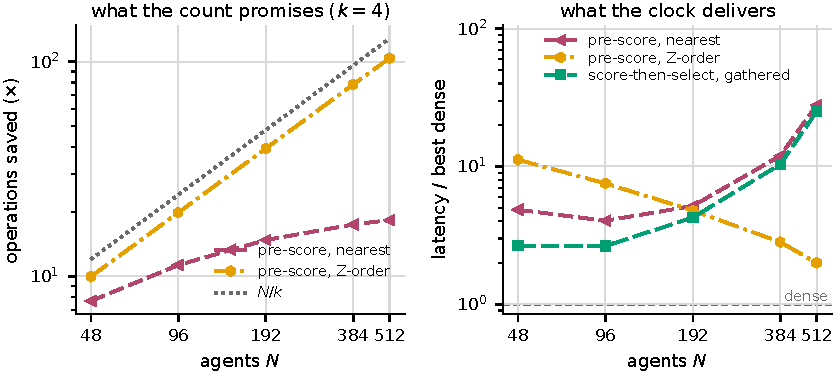
\includegraphics[width=\linewidth]{figures/fig5_prescore.pdf}
\caption{First pre-score sweep. \textbf{Left:} the operation-count saving the
accounting of Section~\ref{sec:escape} promises. The dotted line is $N/k$, the
figure a free selector would reach; the sub-quadratic selector stays below it by
a factor that widens with $N$, and the all-pairs selector is capped by a
constant (Corollary~\ref{cor:taxonomy}). \textbf{Middle:} what the same
configurations cost. Fused, the attention over pre-chosen peers is more than an
order of magnitude faster than dense attention at the largest agent count, and
the total is then governed by the selector, which is where the two selectors
diverge. \textbf{Right:} how far the end-to-end crossing extends. It holds at
two and four retained peers, is level with dense at eight and gone by sixteen.}
\label{fig:prescore}
\end{figure}

Fused, the escape delivers, and how much depends on how many peers are kept. At
two retained peers the attention stage costs $0.60$, $0.44$, $0.19$, $0.08$ and
$0.06$ times dense attention from $48$ to $512$ agents; at four, $0.79$, $0.46$,
$0.24$, $0.12$ and $0.09$. The best case over the grid is $0.060$, sixteen times
faster than dense, at $512$ agents and two retained peers. The advantage narrows
as $k$ grows and is gone at the smallest agent count by sixteen retained peers,
where the stage costs $1.06$ times dense behind the Z-order selector and $1.39$
behind the nearest-neighbour one, whose retained rows are scattered rather than
adjacent. That shape is what the accounting predicts once the score term shrinks
with the aggregation, and no score-then-select implementation in this paper
comes close to it at any sparsity, because none of them can remove the score
term.

Composed from library operators, the same stage is slower than dense attention
at every one of the forty configurations, by $1.03$ to $5.58$ times. Fusing it
is worth between $4.0$ and $17.3$ times, and the factor grows with the agent
count because the gathered tensor the composition writes and re-reads grows with
it. We report both columns because the composed one is what we measured before
writing the kernel, and on its own it supports the opposite conclusion.

End to end the selector decides the outcome, and the two selectors behave
oppositely. The Z-order selector's cost is nearly flat in the agent count ---
$0.102$ to $0.142$\,ms across the range --- so its share of the path falls as
attention grows more expensive: at four retained peers the whole path costs
$13.9$, $8.7$, $3.8$, $1.28$ and $0.85$ times dense attention from $48$ to $512$
agents. The nearest-neighbour selector moves the other way. It materialises an
$N \times N$ distance matrix and ranks it, which is
Corollary~\ref{cor:taxonomy}(b), so beyond $96$ agents its cost grows
quadratically and its path rises to $32.3$ times dense.

The end-to-end crossing at $512$ agents needs a qualification the attention
stage does not. It is a best-case result and it does not survive a change of
estimator. Every latency in this paper is a minimum over interleaved samples, an
estimate of what the configuration costs when the shared device is not being
disturbed. Under that estimator the Z-order path costs $0.83$ times dense at two
retained peers and $0.94$ at eight, and the two runs of the sweep agree to
within $2.3\%$. Under the ratio of medians of the same samples it costs $2.06$
times dense instead. The reason is visible in the dispersion: the pre-score path
is several library kernels behind one selector, and on a contended device the
tail of a multi-launch path is much heavier than the tail of a single dense
kernel, so the median charges it for contention that the minimum removes from
both sides. We therefore report the crossing as an uncontended-envelope result
and make no claim about end-to-end cost under load. The attention stage carries
no such caveat: it is $16.8$ times faster than dense on minima and $15.7$ on
medians.

Three things follow, and together they are the paper's constructive result.

Escaping the operation-count ceiling is necessary and not sufficient. Both
selectors escape it, by between $7$ and $107$ times in operations at
four retained peers, and one of
them is an order of magnitude slower than dense attention while the other is
faster. What separates them is whether the selector reaches its decision through
a structure of the size it was introduced to avoid.
Corollary~\ref{cor:taxonomy} says as much before any measurement: the
nearest-neighbour selector is capped at a constant by its own all-pairs
structure. What the measurement adds is that the cap binds far below its
analytic value, because the selector's cost is traffic rather than arithmetic
and the count charges only the arithmetic.

A cheap selector is not sufficient either. With the attention stage composed
from library operators the Z-order path is slower than dense at every agent
count we measure, and only the fused kernel brings the total to parity at all.
Both conditions are needed, and an operation count expresses neither.

And the regime matters, in a way that limits what this result recommends. The
crossing appears at $512$ agents, the largest count we measure, and we do not
extrapolate past it. Most of the multi-agent communication methods we cite are evaluated with two to roughly thirty agents, and DGN and ATOC with about a hundred (Section~\ref{sec:related}); at those counts our own measurements put
the pre-score path behind dense attention, by $13.9$ times at $48$ agents and
$1.28$ at $384$. So the negative result of Section~\ref{sec:measurement} is the
one that bears on current practice, and this section is a demonstration of a
mechanism rather than a recommendation to adopt this implementation. What it
supplies to a designer is a question with a checkable answer in place of an
appeal to an operation count: whether the selector avoids a structure of the
size it was introduced to remove, and whether the sparse attention it leaves
behind is executed in a kernel written for it.
